We apply our watermark to LLaDA-8b, although the algorithm is applicable to other DLMs \cite{nie2025large}. We randomly select prompts from the ELI5 dataset for evaluation \cite{fan2019eli5}. We generate responses between 100 and 400 tokens, at temperature 0.5. At lengths under 200, detection reliability is worse, as we need sufficient sample size for the binomial test. We measure watermark strength with true positive rate at a 1\% false positive rate threshold (TPR @ 1).

\textbf{Watermark Reliability}
Figure 2 shows that at generation length 400, our algorithm achieves a 97\% TPR @ 1 over 1000 different prompts. At generation length 200, TPR @ 1 drops to 74\%, which is due to the necessity of a sufficient sample size. Figure 3 compares TPR @ 1 at increasing levels of the scaling parameter, $\delta$, with each value of $\delta$ being evaluated on 100 different prompts. We have chosen $\delta$ = 2.0 for our experiments, since it results in high detection rate without as much impact to text quality. 

\textbf{}

\begin{figure}[h]
    \centering
    \begin{subfigure}[b]{0.48\linewidth}
        \centering
        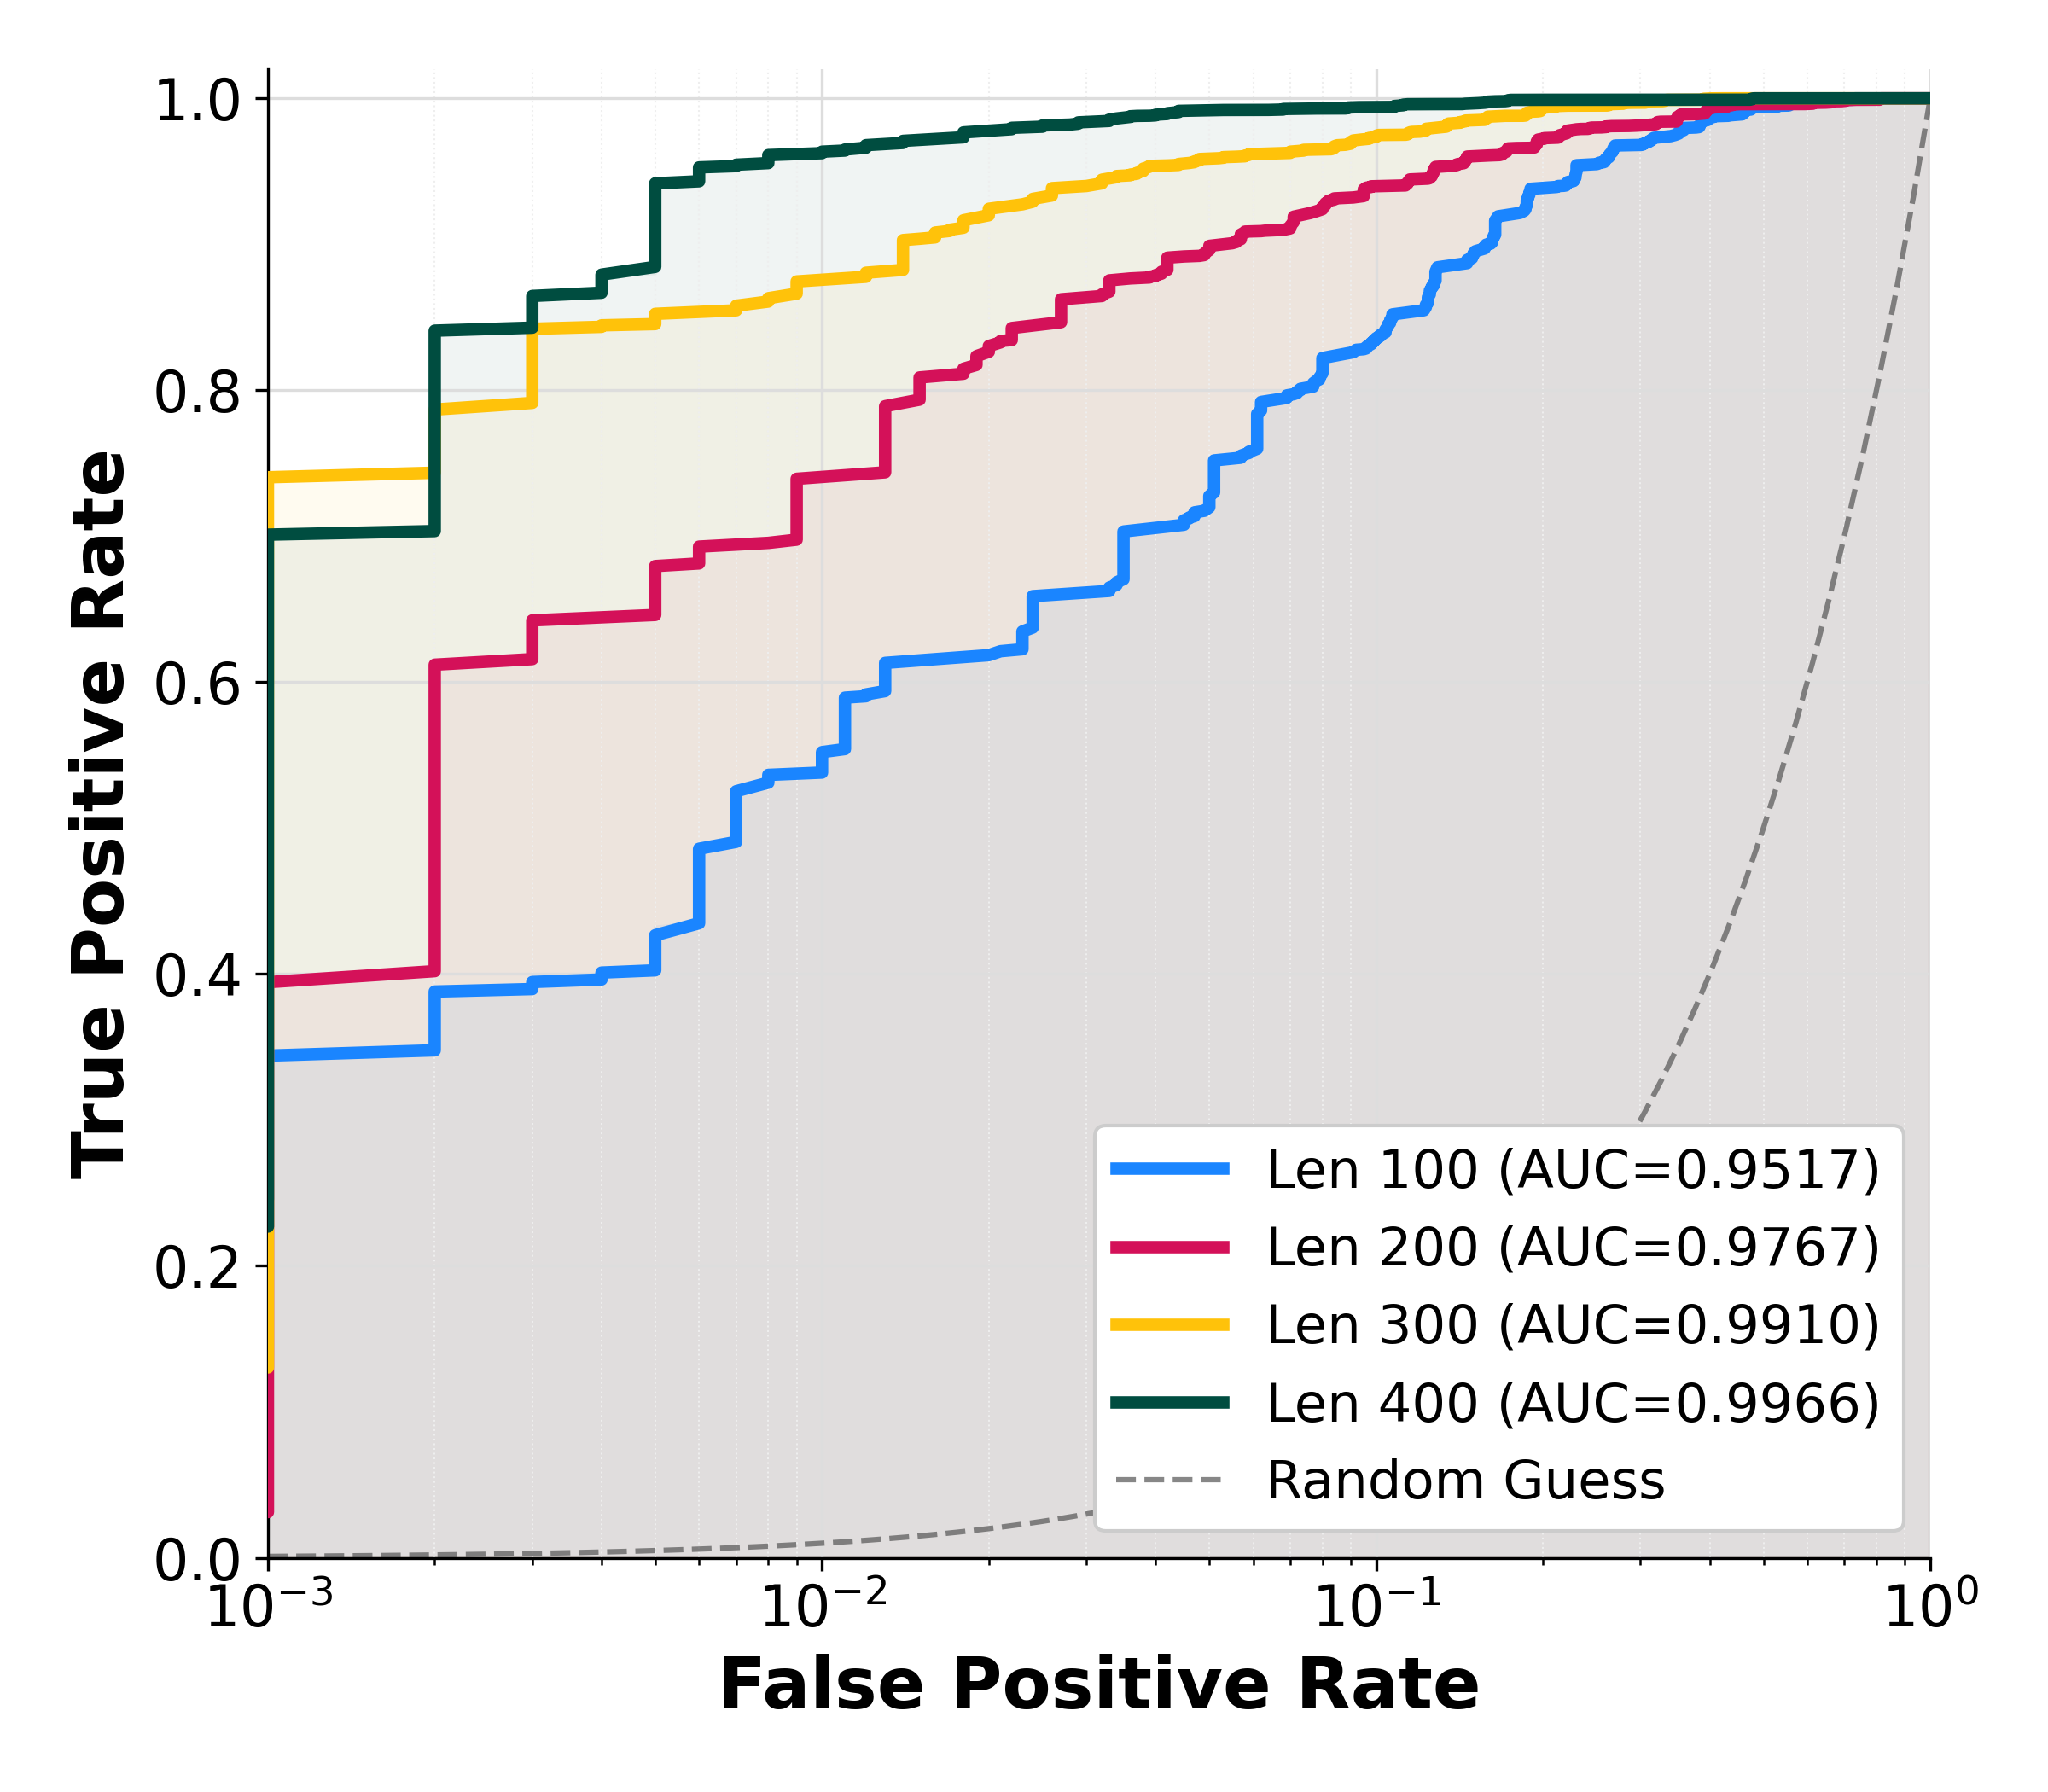
\includegraphics[width=\linewidth]{figures/roc_curve.png}
        \label{fig:roc_length}
    \end{subfigure}
    \hfill
    \begin{subfigure}[b]{0.48\linewidth}
        \centering
        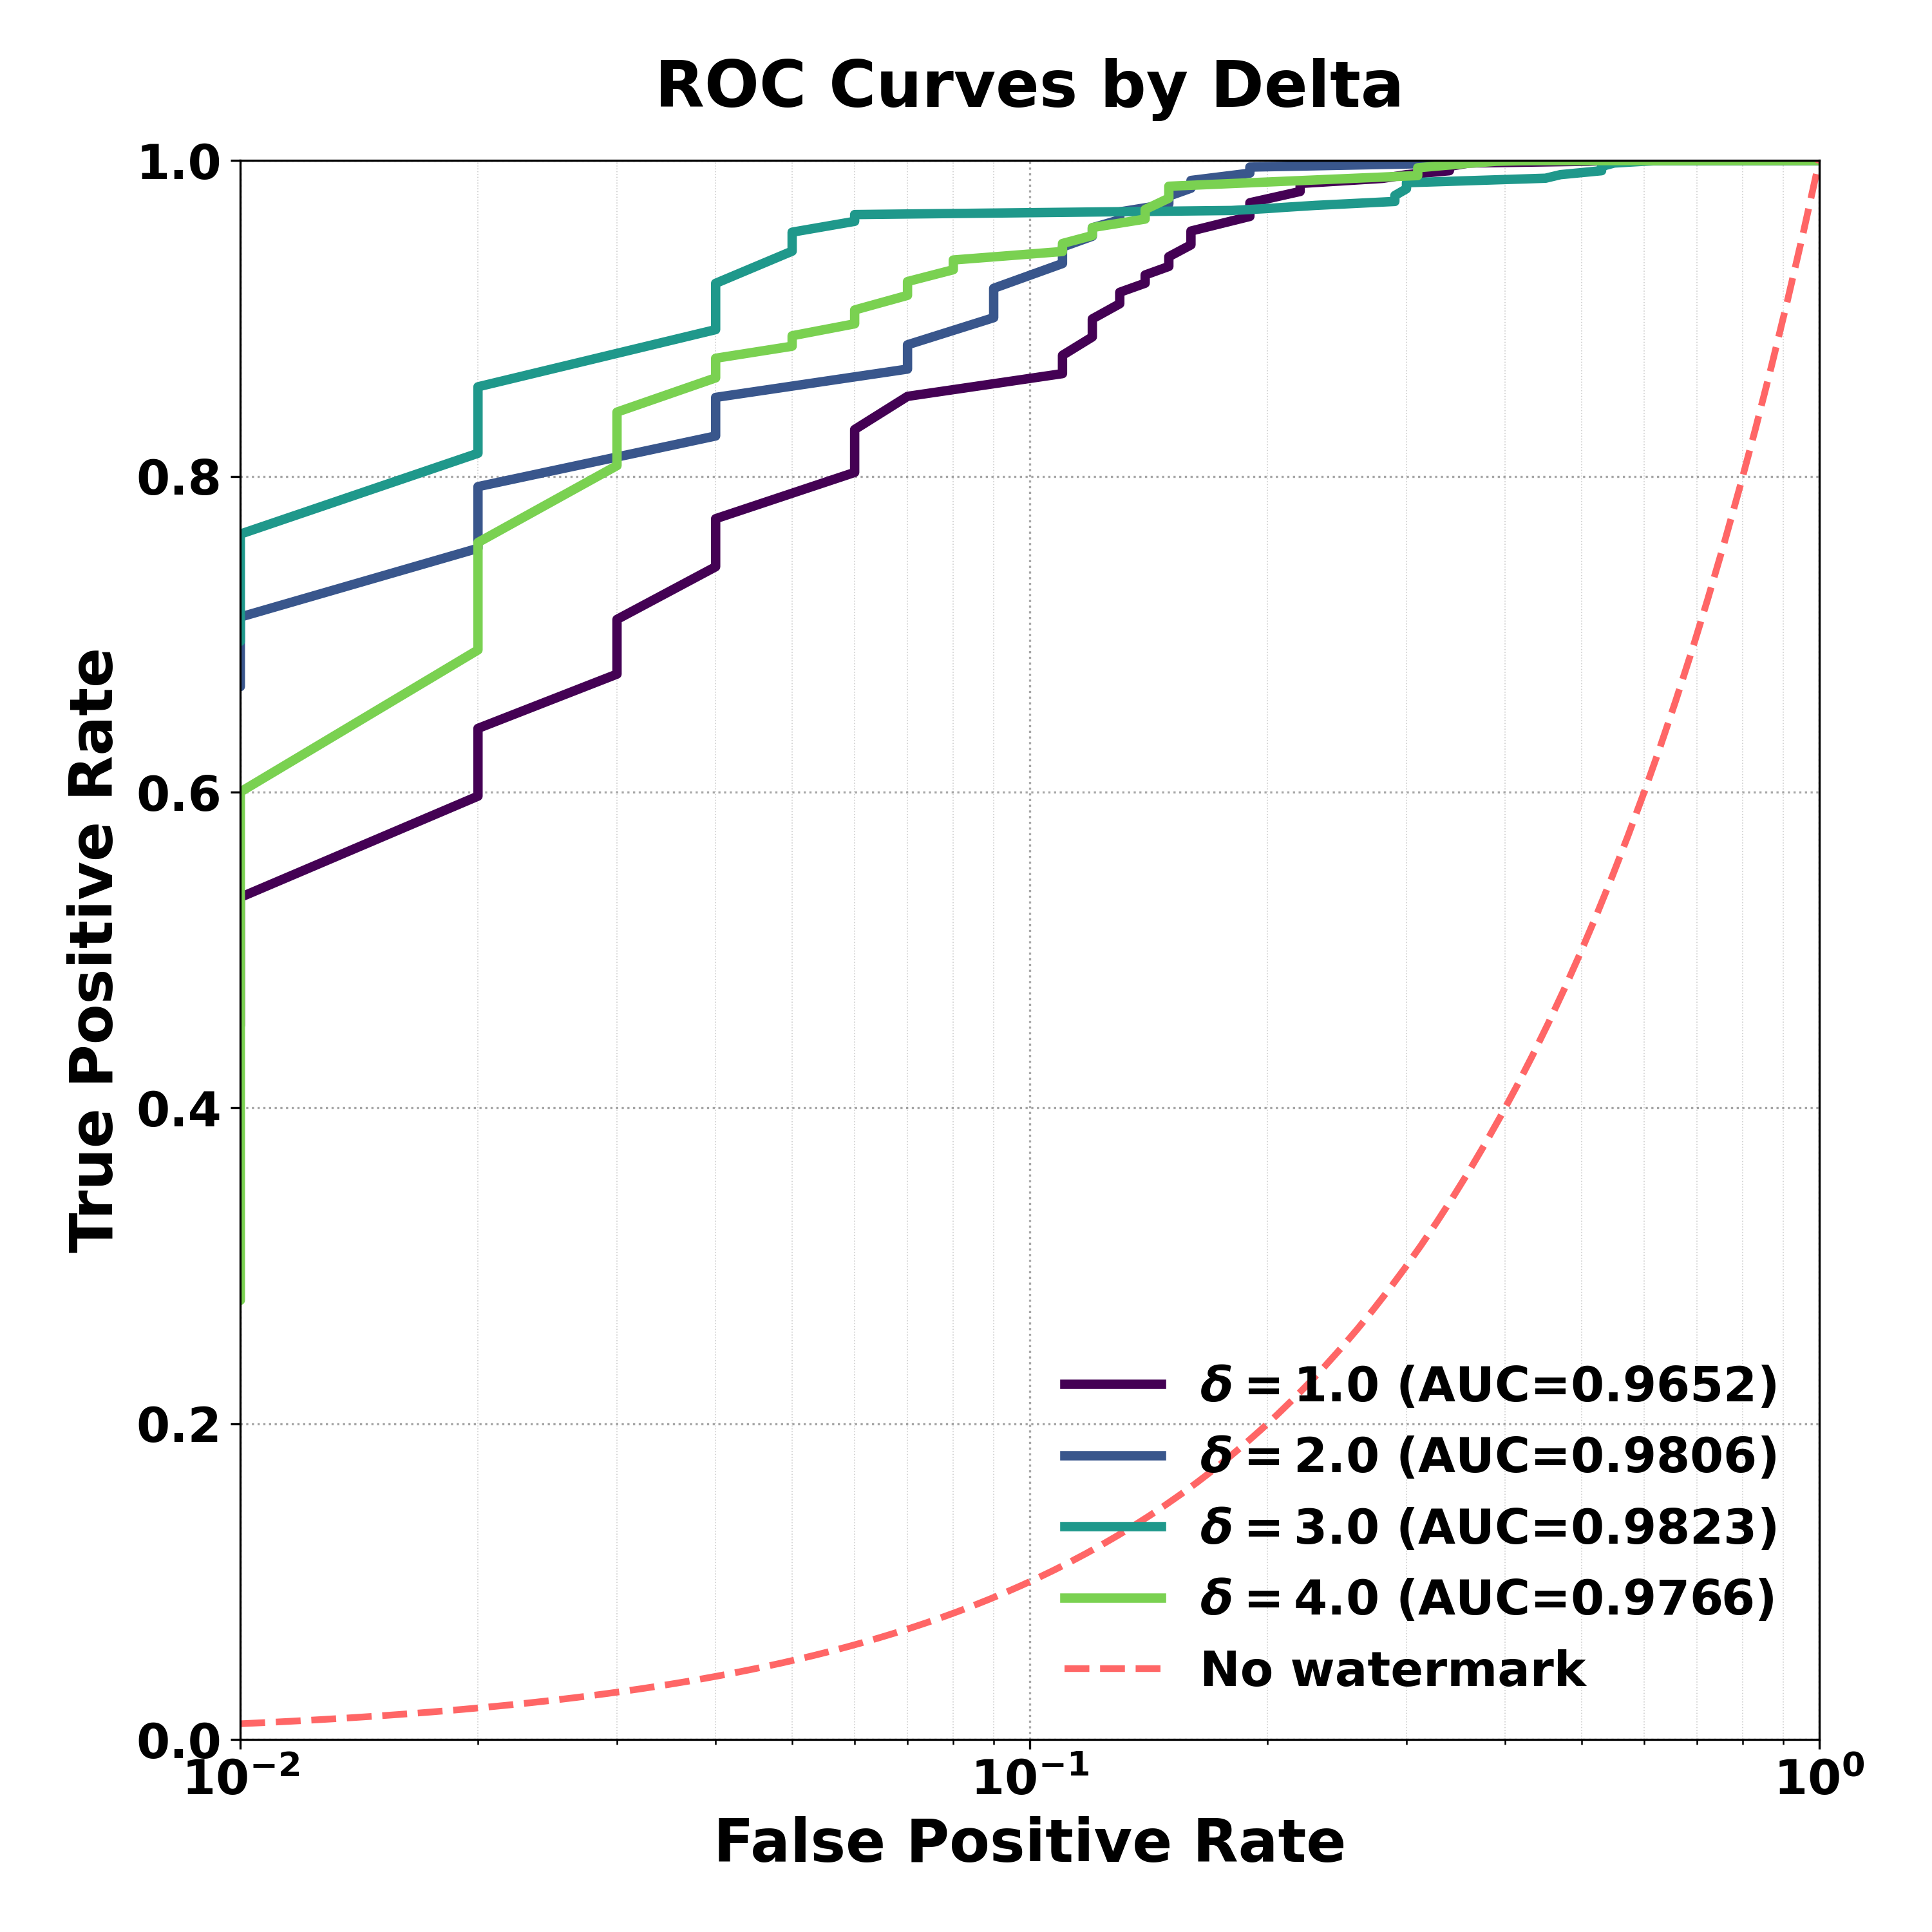
\includegraphics[width=\linewidth, trim=0 0 0 50, clip]{figures/roc.png}        
        \label{fig:roc_delta}
    \end{subfigure}
    \caption{Watermark Performance: ROC Curves Across Deltas and Token Lengths. TPR=FPR plotted in red. (Left) TPR plotted with FPR (1000 samples per length, fixed $\delta=2.0$). (Right) Varying deltas (fixed $N=400$).}
    \label{fig:roc_curve}
\end{figure}
\begin{figure}[h]
    \centering
    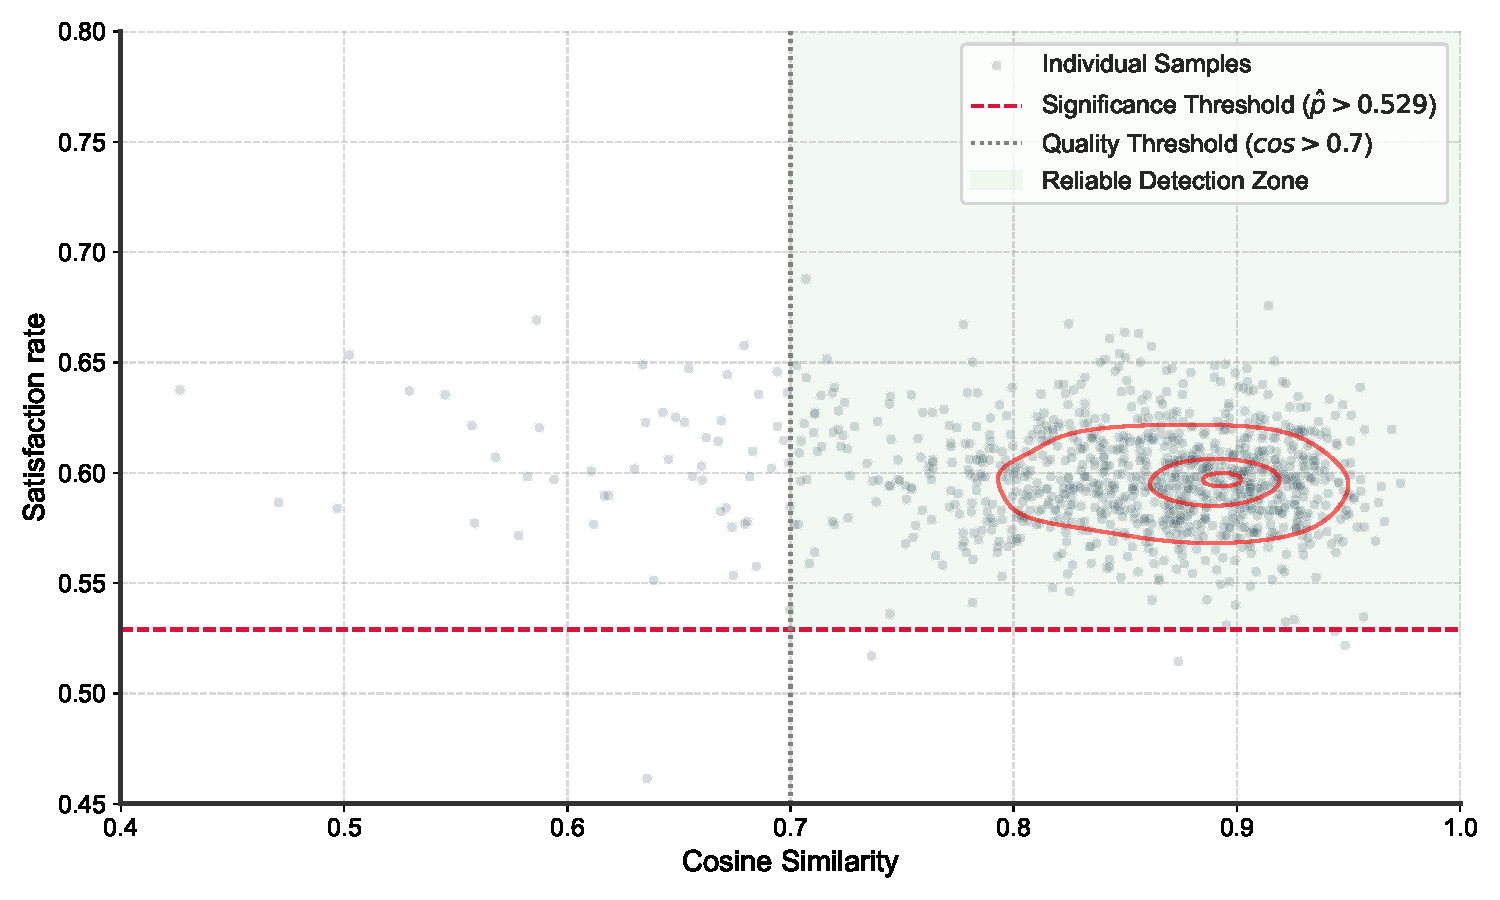
\includegraphics[width=0.8\linewidth]{figures/binomial_signal_analysis.pdf} 
    \caption{Signal Analysis (N=1000). Correlation between satisfaction rate and cosine similarity for outputs of length 400 ($\delta=2.0$). The concentration of samples is shown within the detection region (cos>0.7, $\hat{p}>0.529$), with contour rings at concentrations \{0.99, 0.9, 0.5\}.}
    \label{fig:signal_analysis}
\end{figure}
